\section{Video-text retrieval}
\label{sec:video-text_ret}
Representation Learning (RL) aims to learn compact features of high-dimensonal data (e.g. image, video, audio or document), which has a range of applications in cross-modal context matching. Especially between visual and textual information, it learns to embed the vision and language information into the same latent space, where similarities of different modal features reflect the proximity of their original semantics. \\
The image-text matching task is related to various problems such as Image Captioning (\cite{vinyals2015show, xu2015show, anderson2018bottom}), Image-Text retrieval (\cite{radenovic2018fine, vo2019composing, revaud2019learning}) and Visual Question Answering (\cite{xu2016ask, goyal2017making, anderson2018bottom}), to name a few.
In other scenarios, when one static image cannot provide the full meaning of a concept, which needs the spatio-temporal information from a sequence of images as a video, the video-text matching takes place. 
In the area of video-text retrieval, more and more researchers are paying more attention to RL-based modeling.
Common methods (\cite{lin2014visual, yu2017end, mithun2018learning, miech2018learning, dong2019dual}) utilize popular pretrained word embedding models (Word2vec \cite{mikolov2013efficient}, Glove \cite{pennington2014glove}, etc.) along with sequential models (LSTM \cite{hochreiter1997long}, GRU \cite{cho2014learning}) to construct textual feature extractors. For visual modeling, while some works (\cite{zhang2018cross, miech2020end}) utilize Conv3D based backbones (C3D \cite{carreira2017quo}, S3D \cite{xie2018rethinking}), others use pretrained Conv2D networks to encode frame-level features, and aggregate these features into a video-level representation by a sequential model or pooling function, \cite{li2019w2vv++,ging2020coot}. 
\begin{figure}[t!]
    \centering
    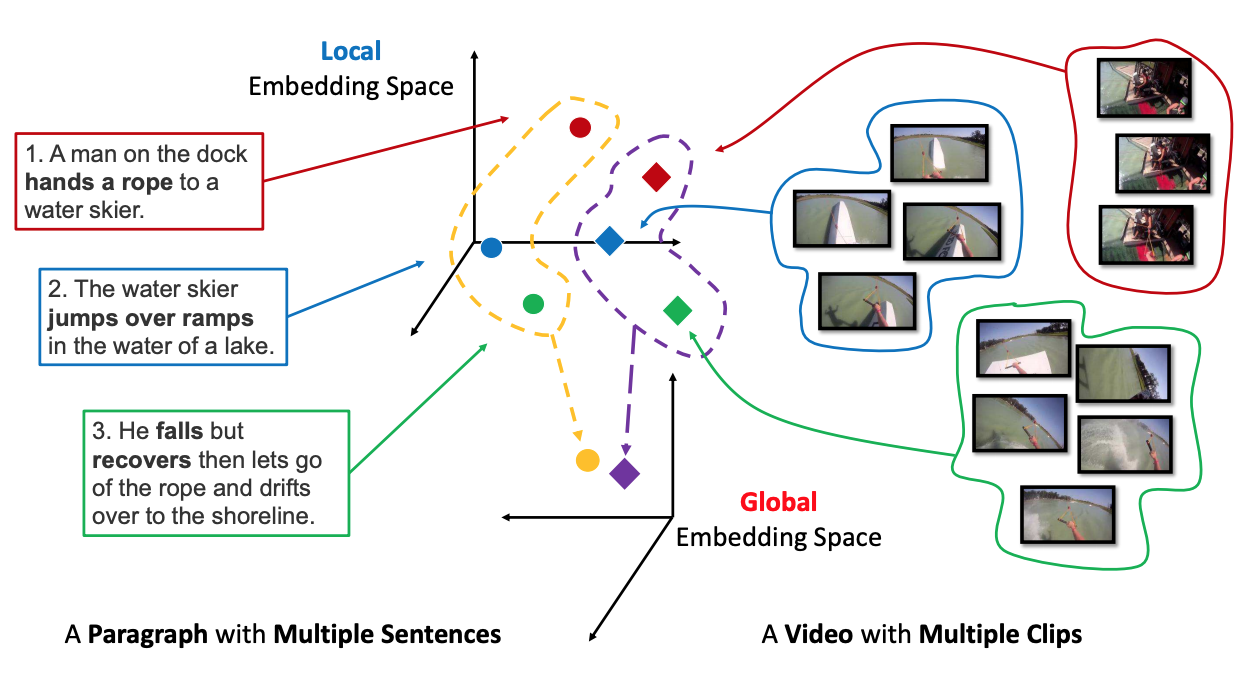
\includegraphics[width=0.9\textwidth]{resources/images/long_vid-text.png}
    \caption{A conceptual diagram illustrates the process of modeling long-range input. The sentence/clip and paragraph/video pair is represented in local and global space respectively. \cite{zhang2018cross}}
    \label{fig:long_vidtext}
\end{figure}
Further, some works deal with long-range video-text relationship, in which video input is a set of consecutive clips, each displays a specific event and text data is a paragraph of multiple sentences describing those events in the respective order. 
Zhang et al. \cite{zhang2018cross} constructs a hierarchical architecture with different levels: video/paragraph, clip/sentence, frame/word to capture the whole temporal context, and apply losses that enforces the interaction between and within different hierarchy levels (shown in Figure \ref{fig:long_vidtext}). Ging, Simon, et al. \cite{ging2020coot} utilizes the objective function from Zhang et al. \cite{zhang2018cross} and proposes a new transformer-based architecture along with a trainable aggregation function to learn better representation. In this work, we adopt these modules to build a RL-based retrieval module, which is also used as a baseline for further improvements.\\
In some cases when the retrieval targets based on some specific details, and the video may contain abundant relations, those aformentioned methods could pay less attention to those important relations, which leads to worse performance. The RL-based architectures now need to enhance those semantic representations when modeling. Feng, Zerun, et al \cite{feng2020exploiting} address the issue by generating region features with semantic relations for frame-level embeddings. Chen, Shizhe, et al \cite{chen2020fine} proposes a hierarchy of three-level semantic matching: event level (based on whole input sentence), actions and entities denoted by verbs and noun phrases respectively. Taking inspiration from these approaches, we propose a relation module to extract semantic relationships between targets and neighboring objects.

